\section{Mitigating the Latency of\newline Programming network state}

The success of many SDN applications hinges on their ability to quickly
program network state. For example:

\minisection{WAN Failover}
When WAN failures occur, an SDN application may want to quickly compute new
paths for flows traversing failed nodes or links, while simultaneously
rerouting other high/low priority flows to avoid hot-spots~\cite{swan}.
However, this requires significant updates to network state at multiple
switches. The longer these updates take, the longer traffic is subject to
congestion and loss. We find that outbound latencies can inflate failure
response time by $\approx$ 20s (\secref{s:evaluation}). 

%\minisection{Failover}
%It is possible that SDN can help mitigate the network-wide impact of
%failures in wide-area networks, reducing both downtime and congestion
%without requiring significant over provisioning. When failures occur,
%the SDN management application can quickly compute new paths for flows
%traversing failed nodes or links, while also simultaneously rerouting
%other high/low priority flows so as to avoid hot-spots~\cite{swan}.
%However, this requires significant updates to network state at
%multiple network switches. The longer these updates take, the longer
%the effect of failure is felt in the form of congestion and drops. We
%find that outbound latencies can inflate the time by nearly 20s
%(\secref{s:evaluation}) putting into question SDN's applicability to
%this scenario. 

\minisection{Intra-Datacenter Traffic Engineering} 
To eliminate hot\-spots and maximize data center performance, an SDN
application may want to reroute traffic subsets at fine
timescales~\cite{hedera}. For example, MicroTE~\cite{microte} leverages the
fact that a significant fraction of ToR-to-ToR traffic (ToR is ``top-of-rack''
switch) is predictable on short time-scales of 1-2s. Thus, MicroTE
frequently computes and updates routes at ToR switches.
% The computed routes may only be effective for 1-2s after which a new sets of
% routes may be more optimal. 
Unfortunately, outbound latencies can cause these updates to take up to 0.5s 
(\secref{s:evaluation}), so traffic that is predictable on 1s timescales is 
optimally routed only half the time.
%Thus, latencies in installing routes can significantly undermine MicroTE's
%effectiveness. Indeed, we find that updating a set of routes at a ToR switch
%in MicroTE can take as long as 0.5s on some SDN switches
%(\secref{s:evaluation}). 

To mitigate the impact of outbound latency, and support the needs of these
and other SDN apps, we propose three immediately deployable
techniques: flow engineering (\FE), rule offload (\RO), and rule reordering
(\RR). This section discusses these techniques in detail; we
evaluate them in \secref{s:evaluation}.

\subsection{Flow Engineering}
\label{s:floweng}

\begin{figure}
\centering
%\begin{minipage}{.45\textwidth}
  \centering
  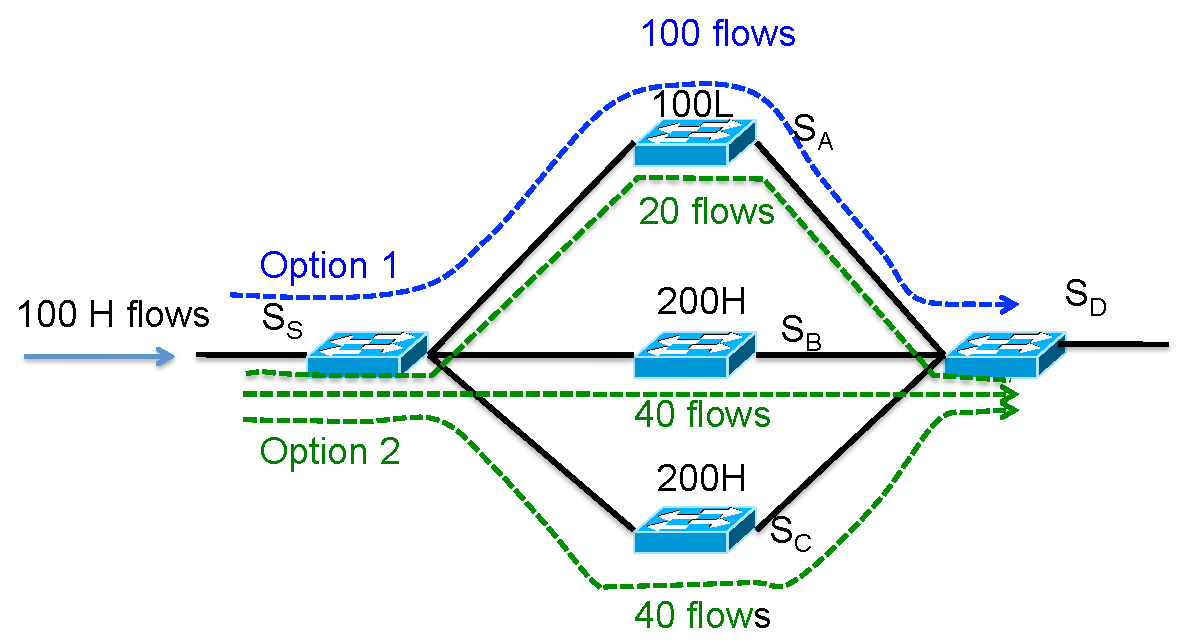
\includegraphics[width=3.2in]{figs/flow_eng_example.pdf} \compactcaption{Flow 
engineering example, assuming \BroadcomOne. $nL$ = $n$ low priority rules;
$nH$ = $n$ high priority rules; capacity = 1000 rules. Ingress and egress 
tables are empty} 
\label{fig:flow_eng} \end{figure}

SDN applications that perform failure recovery, traffic engineering, or other
forms of routing must quickly compute and setup network paths in order to
satisfy reachability and performance objectives. These applications must often
select one of many possible paths based on congestion, delay, flow table 
occupancy, or other metrics. Unfortunately, a (slightly) more optimal path 
according to these metrics may take significantly longer to setup due to 
outbound latency.

For example, consider an SDN application that seeks to minimize the
imbalance in flow table occupancy~\cite{swan, simple, minlanvcrib}. If such an
application needed to setup routes for 100 flows of high priority $H$ in the
topology shown in Figure~\ref{fig:flow_eng}, it would select the first path
through switch $S_A$ for all flows, thereby equalizing the number of flow
table entries across all switches. However, assuming the switches are
\BroadcomOne, this would require displacing {\em each} of the 100 existing
rules of low priority $L$ in $S_A$ for {\em each} of the 100 new flows,
resulting in a total flow installation time of $\approx$1.5s. In contrast, by
routing only 20 new flows through $S_A$, and dividing the remaining flows
evenly between the paths through $S_B$ and $S_C$, we can keep the same level
of imbalance in flow table occupancy ($S_B$ and $S_C$ each have twice as many
entries as $S_A$), while reducing the total flow installation time to
$\approx$0.3s (assuming rules are installed in $S_A$, $S_B$, and $S_C$ in
parallel). 


%SDN applications typically compute paths between various network
%locations that meet some global objective pertaining to
%performance or security. A common issue considered in most prior works
%on such applications is to deal with limited switch table sizes, by
%picking routes that obey or optimize table space
%constraints~\cite{swan,simple, minlanvcrib}. Unfortunately,
%these techniques do not provide sufficient control over outbound
%delay. 

%\minisection{Minimize maximum flow table occupancy is very suboptimal} 
%For example, consider a simple setting where there are three candidate
%paths between a pair of nodes as shown in Figure~\ref{fig:flow_eng}.
%Each path has one Broadcom switch. The switch on the first path
%has 100 rules of low priority L, whereas the switches on the second
%and third paths each have 400 rules of high priority H. Suppose that a
%hypothetical traffic engineering application has 100 flows of priority
%H to allocate to these paths, and each path is equally preferable
%for a flow.  Existing techniques for table space management would
%assign all flows to the first path to minimize maximum flow table occupancy; but
%our measurements for Broadcom 
%show that {\em each} of these 100 rules will displace
%all the 100 low priority rules in the TCAM, resulting in high
%latencies! Allocating 50 flows each on the
%latter two paths instead results in no rule displacement, and the number of
%rules installed per path will be smaller. Thus, when the flows are installed in
%parallel across the latter two paths, this results in significant reduction in
%installation latency. Based on Figure~\ref{fig:burst-completion-time}, it is about 200 ms
%vs 2 seconds, a 10X difference. 
%%Intel switches have similar issues, but for other priority patterns.
%%li: yes, according Marina's information. Low priority rule displaces high
%%priority rule depending on their location.
%%\aditya{check intel claim}

The goal of {\em flow engineering} (\FE) is to select paths that minimize
installation delay while still satisfying an SDN application's primary path
selection criteria (e.g., flow table occupancy or congestion). Assuming there
are many possible sets of paths $\{\mathcal{P}^i_{obj}\}_i$ that (closely)
satisfy an application's objectives, FE selects the set
$\mathcal{P}^{displace}_{obj,tbl\_sz}$ that minimizes the aggregate
latency impact of rule installations, and any associated rule displacements,
while still obeying flow table space constraints.
%The goal of flow engineering is to select paths across the network
%such that installation delay is minimized. The key insight we use is
%the following: in general, there are many possible sets of paths
%$\{\mathcal{P}^i_{obj}\}_i$ in a network that optimize an SDN
%application's objectives, e.g., optimal capacity and latency. From
%this, flow engineering selects the set
%$\mathcal{P}^{displace}_{obj,tbl\_sz}$ that minimizes the aggregate
%impact of both rule displacement in TCAM as well as the number of rules
%installed at any switch, while obeying table space constraints.
% maximum number of rules installed at any
% switch; thus, we spread rule update load {\em laterally}, helping
% improve outbound latencies.
%
$\mathcal{P}^{displace}_{obj,tbl\_sz}$ can be computed using a two step
optimization:
({\em i}) identify sets of paths that satisfy the SDN application's objective 
function,
%\aaron{What is ``the network's objective function?''}
but do not select the actual
paths to use; ({\em ii}) select paths that minimize aggregate
flow installation time.
%effect of rule displacement and the number of rules to be inserted at any
%switch.  
Unfortunately, the time required to solve the integer linear program
(presented in  \appref{app:floweng}) would
outweigh the latency benefits it seeks provide, so we formulate an
efficient heuristic.
%The detailed optimization formulation is a large integer linear
%program (omitted for brevity) and hence inefficient to solve. Below, we
%discuss a simplifying heuristic in the context of a traffic engineering
%application.

\minisection{Flow Engineering Heuristic}
Our goal is to satisfy a bound $C$ on the time required to install/modify
rules across all switches. 
%We initialize $C$ to a low value.

We represent the network as a graph $G = (V,E)$, where each node is a switch
(or PoP) and each edge is a link (or tunnel). Given a traffic matrix $M$, the
SDN application computes $K$ candidate equal cost paths for each $(u,v) \in
V$, where cost is defined in terms of the application's objective (e.g.,
average link utilization). We assume the application also assigns a priority
$Pri(u,v)$ to each flow $(u,v)$.

%\aaron{This is very specific to the objective of minimizing average link
%utilization; can we make this more generic?} 

We sort the flows in decreasing order of resource demand (e.g., bandwidth) and
iterate through them. For each flow $(u,v)$ in the sorted order, we consider
the corresponding $K$ equal cost paths in decreasing order of resource 
availability; let $P^{1\ldots K}_{(u,v)}$ be the sorted order. If the resource
demand $d_{uv}$ can be satisfied by the path $P^{1}_{(u,v)}$, then we compute
whether installing/updating rules for flow $(u,v)$ along this path violates the
latency bound $C$.

%We do this by modeling the per-switch latency, as well as maximum latency
%on the path:

%We represent the network as a graph \textit{G = (V,E)}, where each node is a
%switch (or PoP) and each edge is a link (or tunnel). Given
%a traffic matrix $M$, the application attempts to route it such that the
%average link utilization is within some bound; the heuristic can be easily
%extended to accommodate other objectives.
%% Our goal to compute routes such that the objective is maximized as well as
%% the cost of installing the necessary rules at switches is minimized. 
%%Our heuristic works by exploring for each source-destination pair
%For each source-destination pair we see, whether a path can accommodate both
%its demand, and the path setup latency  
%%imposed by routing the pair across the path's switches 
%is within some bound. If either is violated, we try the next candidate path.
%
%More precisely, suppose we want to bound the maximum cost of
%installing rules at any switch by some $C$. We start by selecting some
%low value for $C$. We assume that we have computed $K$ candidate equal cost
%paths for each $(u,v) \in V$. Suppose the priority of the $(u,v)$ flow
%is $Pri(u,v)$ at every switch in the network (this is
%typically set by the operator).
%
%We sort the traffic demands in decreasing order and
%iterate through them. For each $(u,v)$ in the sorted order, we
%consider the corresponding $K$ equal cost paths in decreasing order
%of available capacity; let $P^{1\ldots K}_{(u,v)}$ be the sorted order. 
%
%If the demand $d_{uv}$ can be satisfied by the path $P^{1}_{(u,v)}$ within
%the utilization bound, then we compute whether installing the $(u,v)$ path
%violates the rule installation latency bound or not. We do this by modeling
%the per-switch latency, as well as maximum latency on the path:



%\minisection{Per-switch latency}
% Recall that we always install new rules,
%and never do rule modifications and deletions. 
%\aditya{the previous sentence may have to go}
% In doing this, an issue to consider is whether the rule for
% $(u,v)$ at $s$ is modifying an existing forwarding rule for $(u,v)$ at
% $s$ (this would happen if $(u,v)$ was being routed through $s$ before,
% but the next hop from $s$ has now changed) or it is a new rule being
% inserted (this happens if $(u,v)$ was never routed via $s$ before).
% However, recall that our measurements show that modifying a rule is
% much more expensive than inserting a new rule (the former incurs the
% cost of potentially reshuffling the entire existing set of rules at
% the switch, whereas the latter only displaces lower priority rules).
% Therefore, we {\em always insert} a new rule for $(u,v)$, ensuring
% that the rule is of higher priority than the existing rule for $(u,v)$
% in $s$ (if any). 
Given our measurement results, for every switch $s \in P^{1}_{(u,v)}$, we can
model the latency at $s$ due to installing rules for $(u,v)$ as 
$L_s = \max(a, (b +c * Disp_s(Pri(u,v))))$. Here, $Disp_s(Pri(u,v))$ is the 
number of rules at $s$ that will be displaced by the rule for $(u,v)$.
%% the following discussion is not very useful, it seems 
%For the Broadcom switch, this is the number of rules of priority {\em lower}  than $Pri(u,v)$, whereas for the Intel switch
%$Disp_s(Pri(u,v))$ is the number of rules of priority \emph{higher} than
%$Pri(u,v)$ divided by 300. 
%This is a conservative estimate assuming all rules
%are packed in increasing priority of slices (\S\ref{s:meas_insert}).
%\aditya{check intel claim} 
%$Disp_s(Pri(u,v))$ can be easily tracked by the SDN
%controller. In the above, 
$a$, $b$ and $c$ are constants derived from switch
measurements. This model essentially says that if the current rule
does not displace any rules from $s$'s existing table, then it incurs
a fixed cost of $a$; otherwise, it incurs the cost given by $b +c *
Disp_s(Pri(u,v))$. The fixed cost $a$ is the insertion delay without any TCAM
reordering. 

%$a$ is the same whether it is modification or insertion for Intel. For
%Broadcom, since we avoided modification, it represents insertion delay without
%TCAM displacement. 
%\aditya{refer back to the model from
%  the measurement section}

%\minisection{Maximum installation latency} 
Now, $\forall s \in P^{1}_{(u,v)}$, we check if $L_s + CurrentL_s \le C$,
where $CurrentL_s$ is the current running total cost of installing the
rules at $s$, accumulated from vertex pairs considered prior to $(u,v)$ in our
iterative approach.
If this inequality is satisfied, we assign $(u,v)$ to the path
$P^{1}_{(u,v)}$ and move to the next vertex pair. If not,
%meaning that installing the $(u,v)$ route on this path violates the
%maximum cost bound $C$ for some switch on the path, then 
we move to the next candidate path for $(u,v)$, i.e., $P^{2}_{(u,v)}$ and
repeat the process.

If after iterating through all flows once, we have not selected a feasible
path for each flow, then we increase $C$ and start from the beginning.
Alternately, we could do a simple binary search on $C$. 
%li: no space for that.
%\aditya{do we need pseudocode?}

%\aditya{assumption: we have a small number of rules we are adding.
%  otherwise, if we can confirm that the decreasing priority weirdness
%  does not apply for all table occupancies, then we should use that}
%\aditya{seems like bcm is buggy so we may not need the above
%  assumption}

% We assign each edge a cost that is the reciprocal of its current available capacity, and find the 
% minimum cost path for the traffic demand. For finding the minimum cost path, we consider precomputed K equal hop length paths, and find
% the path which gives the minimum cost. As we assign a path for a particular traffic demand, 
% we reassign the cost by decreasing the current capacity by the traffic demand for each edge belonging to the
% min-cost path. The idea is that edges which are more highly utilized will get a higher cost value and so the min-cost path for remaining 
% traffic demands will prefer the edges which are lightly utilized. This way, 
% we minimize the maximum load. We analyze the runtime complexity of the algorithm. 

% 
\begin{table}
\begin{scriptsize}
\begin{tabular}{c|l}
Notation & Meaning \\
\hline
$S$ & Set of all switches
\\$S_{ToR}$ & Set of all ToR switches
\\$\tau_{u}$ & Maximum number of flow entries in the switch $u \forall u \in S$
\\$E$ & Set of all physical links (between two adjacent devices)
\\$C_e$ & capacity of individual links $\forall e \in E$
\\$F_{uv}$ & set of all flows from $u$ to $v$ where $u,v \in S$
\\$P_{uv}$ & Set of paths from device $u$ to device $v$
\\$K _{uv}$ & Number of paths from device $u$ to $v$ where $u,v \in S$ 
\\$P^k _{uv}$ & Set of links of $k^{th}$ path from device $u$ to $v$ where $u,v \in S$
\\$T ^f _{uv}$ & Traffic volume from $u$ to $v$ of flow $f$ where $u,v \in S$
\\$util$ & maximum link utilization
\\$I ^{fk} _{uv}$ & Indicator variable denoting that flow $f$ from $u$ to $v$  takes the $k^{th}$ path.
\\$cost$ & maximum cost of rule installation at any switch
\\$M$ & priority of all new rules being inserted
\\$L_s(M)$ & number of rules at switch $s$ of priority lower than $M$
\\ $a$ & cost of installing a rule it has same priority as rules in table
\\ $b$ & constant factor used in modeling rule displacement cost.
\end{tabular}
\label{tab:notation1}
\caption{Notation used in flow engineering formulation.}
\end{scriptsize}
\end{table}

We explain how flow engineering works for simple traffic engineering SDN
application. We represent
the network as a graph \textit{G
  = (V,E)}, where each node is a switch (or a PoP) and each edge is a physical link (or virtual tunnel). Given a traffic matrix, the application attempts to route it such that the maximum link utilization is minimized. Upon computing routes, the application determines the rules to be installed at individual switches. 

For simplicity, we assume that all the rules to be inserted are of the same priority $M$.  We also assume that the control application knows how many rules in each switch have priority lower than $M$, i.e., $L_s(M)$. This can be easily tracked based on history of rule insertions. The notation we use is shown in Table~\ref{tab:notation1}.


{\bf Step 1 - Network Objective:} In the first step we minimize the
maximum link utilization. Let $T ^f _{uv}$ be the traffic volume
 of flow \textit{f} between $(u,v)$, $P^k _{uv}$ be the set of links on
the $k^{th}$ path between (\textit{u,v}). We use a
binary indicator variable $I ^{fk} _{uv}$ to show whether the flow $f$
is on path $k$ or not.  $K _{uv}$ denotes the number of equal hop
length paths between $(u,v)$. 

We have the following capacity constraint: 

% Following are our two
% constraints. First, The total traffic volume from an edge should not
% exceed its $C_e$ times the link utilization limit, $util$. 

\begin{scriptsize}	
\begin{equation*}
    \sum _{u,v \in S_{ToR},~f \in F_{uv},~k  \in P_{uv}~s.t.~e \in P^k _{uv}} T ^f _{uv} *  I^{fk}_{uv} \leq util \times C_e 
\end{equation*}
\end{scriptsize}	
	
The following ensures each flow $f$ takes a single path:	

\begin{equation*}
    \sum _{k  \in P_{uv}} I^{fk}_{uv} = 1 ,\quad \quad \forall u,v \in S_{ToR},~ f \in F_{uv}
\end{equation*}
 
The objective is to minimize the \textit{util}. Note that we do not
compute paths in this step, just the value of the objective function;
suppose the optimal value is $util^*$.

{\bf Step 2 - New Rule Objective:} In second step, we select routes
so as to minimize the rule installation latencies at any
switch. We allow some slack wrt meeting the utilization objective; denote it by
$\delta$. While the second constraint above remains, the capacity
constraint changes to:
 
% First,  traffic traversing from an edge $e$ does not exceed the $C_e$ multipled by 1 $+$ $\delta$ times the $util^*$. $util^*$ is the maximum link utilization we got from the step 1, and  $\delta$ defines an upper limit on maximum link utilization.

\begin{scriptsize}
\begin{equation*}
    \sum _{u,v \in S_{ToR},~f \in F_{uv},~k  \in P_{uv}~s.t.~e \in P^k _{uv}} T ^f _{uv} *  I^{fk}_{uv} \leq (1 + \delta) \times util^* \times C_e 
\end{equation*}
\end{scriptsize}

% We have a similar constraint as above for   Second constraint is same as step 1.\\
  
% \begin{equation*}
%       \sum _{k  \in P_{uv}} I^{fk}_{uv} = 1 ,\quad \quad \forall u,v \in S_{ToR},~ f \in F_{uv}
% \end{equation*}
 % \begin{alignat*}{2}
  %                     & latency = a * entries + c \\
   %                    \text{   where }a \text{ and }c\text{ are constant}\\ 
  %\end{alignat*}

When a rule installed at a switch cause existing lower priority rules to be displaced, we incur a cost that grows linearly with the number of displaced rules, i.e., $b * L_s(M)$, where $b$ is a constant. This cost adds up linearly when a burst of rules is installed. When the burst of rules installed all have the same priority as rules already in the table, we incur a smaller fixed cost per rule, denoted by $a$. Based on this, we track the total cost of rule installation at a switch as follows:
%  for each rule installed at the switch, we incur a cost of we incur a co
% here, we assign a weight ``$a$'' to the number of rules installed and a weight ``$b$'' to the number of rules that need rearrangement:
\aditya{need to make sure we have justification for
  this linear function. provide constants based on measurements.}

\begin{scriptsize}
\begin{equation*}
                       \sum_{u,v \in S_{ToR}, ~f \in F_{uv}, ~k \in
                         P_{uv} ~s.t.~ s\in P^k_{uv} } max(a, b * L_s(M)) I^{fk}_{uv}  +
                       \leq cost \quad \quad \forall s \in S
\end{equation*}
\end{scriptsize}

The objective is to minimize $cost$.   
  



% This can be viewed as solving the following two optimization problems
% in sequence:

% \[
% \begin{array}{lll}
% \text{Problem 1:} & \text{optimize} & NetworkObjective \\
% & \text{subject to} & RuleCapacities \\
% \end{array}
% \]

% \[
% \begin{array}{lll} 
% \text{Problem 2:} & \text{optimize} & NewRuleObjective \\
% & \text{subject to} & NetworkObjective \text{, and, } \\
% & & RuleCapacities
% \end{array}
% \]

% Here $NetworkObjective$ is the SDN application's network wide
% objective function, such as maximum link utilization, $RuleCapacities$
% represent switch table capacities in the network, and
% $NewRuleObjective$ an objective function pertaining to new rules
% inserted at any switch, such as the maximum number of such rules. The
% first optimization problem simply computes the value of the objective
% function, e.g. the maximum link utilization, subject to switch table
% capacity constraints; no actual paths are computed. The second
% optimization problem uses this value as a constraint to compute
% $P^{flowmod}_{obj,tablesize}$.

\minisection{Limitations} Because paths are computed by the SDN application, FE
must be integrated with the application. FE does not apply to scenarios where 
route updates are confined to a single location, presenting no opportunity to
spread update load laterally. One such example is MicroTE~\cite{microte},
where changes in traffic demands are accommodated by altering rules at the
source ToR to reallocate ToR-to-ToR flows across different tunnels.

\iffalse
{\bf Interaction with Update Semantics:}
Flow engineering has to be designed carefully when
management applications are trying to realize various consistency
properties for their updates~\cite{mahajan13:hotnets}. We explain
using examples below.

If updates of network state from ``old'' to ``new'' are not
orchestrated carefully, a variety of consistency issues can arise:
e.g., there may be forwarding loops, or packets may be forwarded
inconsistently (using old state some times and new state at other
times) at different network hops. Both issues are transient, and flow
engineering (as well as the rule offloading and priority ordering
techniques we describe below) can reduce the duration of such loops
by bounding the time that any network switch spends updating
its state.

In practice, some network operators may want to ensure some semantics
for their updates. One example is packet
coherence~\cite{mahajan13:hotnets}, which means
a packet should see consistent state (always old, or always new) as it
traverses the network. This can be achieved using global version
numbers and one-shot updates~\cite{consistentupdates}: (a) new
forwarding state is added to the core of the network, keeping older
state around; (b) the edge is updated to use the new state only when
all core switches confirm the installation of the new state; prior to
this all forwarding happens using old state; (c) old state is removed
from the network only when there are no more packets forwarded using
it. Flow engineering as formulated above directly helps in this case
by speeding up step (a). 

Consider another example semantics, loop freedom; this can be achieved
by ensuring that switches downstream on a new forwarding path are
updated, and their new state used for forwarding, before those
upstream~\cite{mahajan13:hotnets}. In this case, naively applying flow
engineering as specified above may hurt: because it may increase the
number of switches and paths being updated it may correspondingly
increase the aggregate number of ``dependencies'' to track amongst
different switches' updates, slowing down loop-free updates.
Furthermore, spreading of updates across multiple paths can also
introduce dependency cycles; expensive mechanisms are necessary to
break these cycles~\cite{mahajan13:hotnets}. which further slow down
the update. Thus, the total latency of doing a loop-free update can be
significantly higher with naive flow engineering.

We must therefore design appropriate flow engineering schemes for
different update protocols. We leave a full exploration of this issue
for future work. Where the issue arise, we assume the network is using
one-shot updates.

\aditya{lead out}

\fi

%\subsubsection{MicroTE}

% LocalWords:  Broadcom SDN TCAM rearrangment tbl sz PoP Pri uv Disp CurrentL
% LocalWords:  MicroTE ToR

\subsection{Rule Offload}
\label{s:offload}

\begin{figure}
\centering
%\begin{minipage}{.45\textwidth}
  \centering
  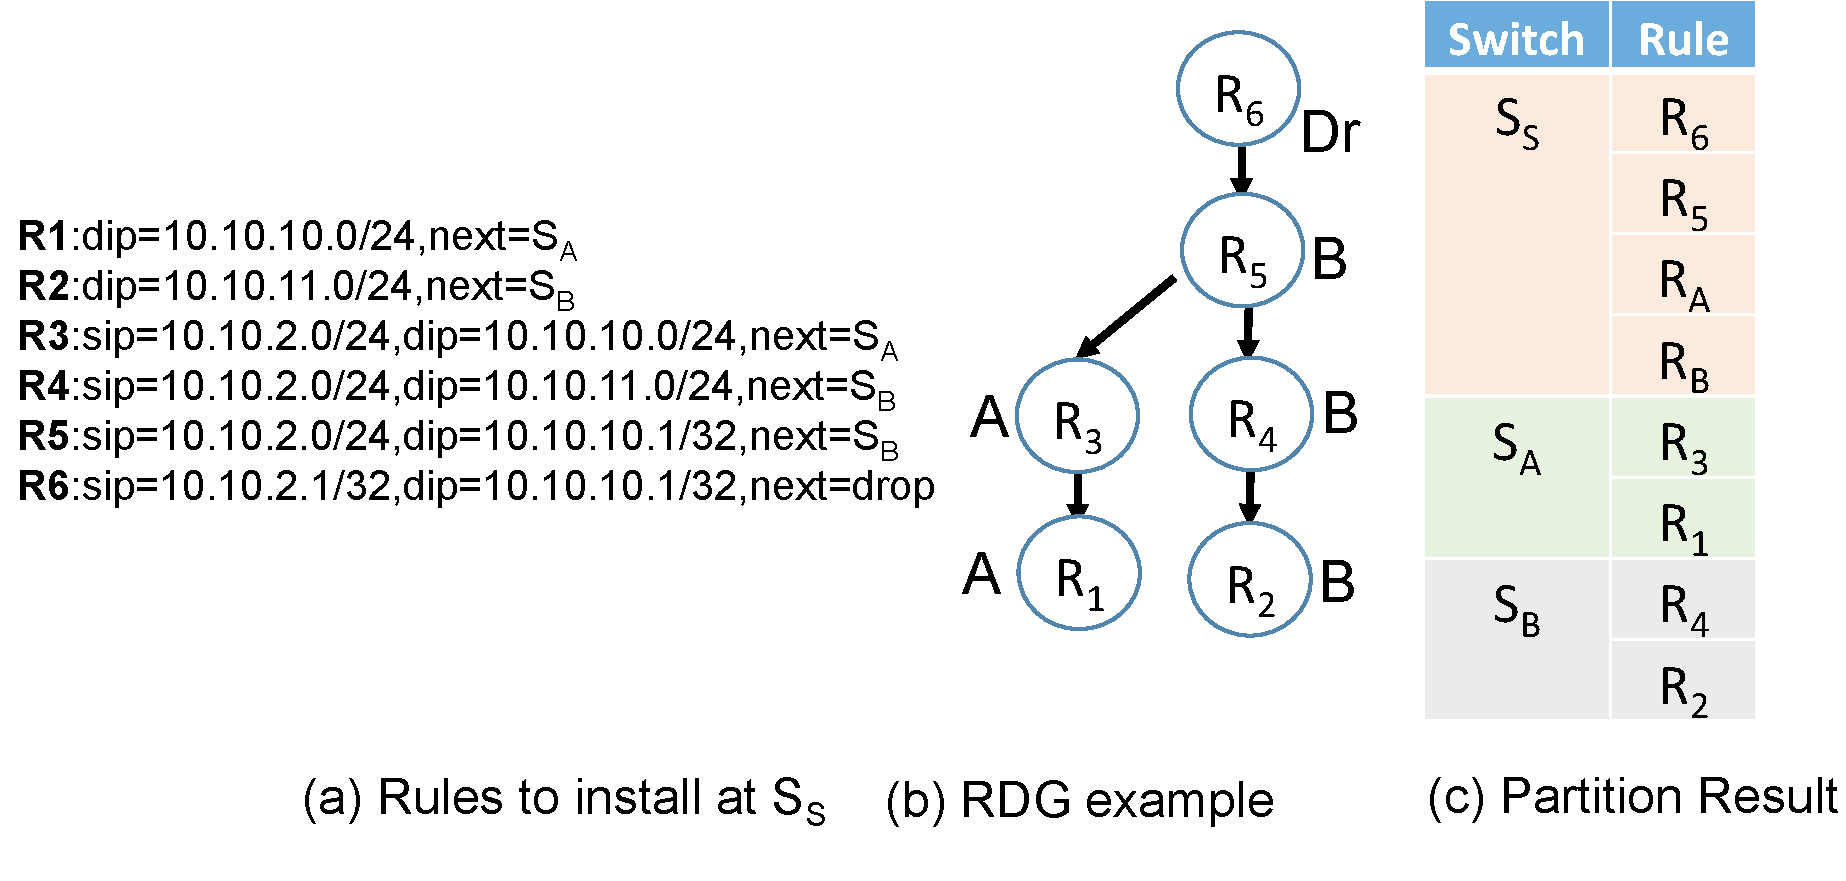
\includegraphics[width=3.0in]{figs/Rule-Offload2.pdf}
\compactcaption{Rule offloading example}
\label{fig:rule-offload}
\end{figure}

%\aditya{LI: this section does not talk about differences wrt difane, vcrib. li, can you fix?}
%\aditya{LI: we should also talk about encapsulation on the core router}

When FE selects a path for a set of flows, the same number of rules are
installed/modified in every switch along the path. Thus, a path's update
latency is determined by the switch with the largest number of existing
low priority rules (assuming \BroadcomOne), or the largest number of pending
rule installations/modifications. For example, since switch $S_S$ in
\figref{fig:flow_eng} is part of all three paths to reach switch $S_D$, a
rule must be installed in $S_S$ for every new flow, regardless of whether the
flow traverses the path through $S_A$, $S_B$, or $S_C$.  Assuming
\BroadcomOne switches, it will take at least 0.3s to install rules for 100
flows of high priority $H$ in $S_S$---the same time required to install 20
rules in $S_A$ and longer than the $\approx$0.12s required to install 40
rules in both $S_B$ and $S_C$.


%Rule offloading applies particularly to networks where tunnels are
%used, e.g., cellular networks (\S\ref{sec-motivation}), carrier networks
%that rely on label-switching, data centers using VXLAN
%%~\cite{xxx} \aditya{check this} 
%and inter-DC WAN networks such as those considered
%in~\cite{swan,b4}. In such networks, SDN applications
%control the tunnel end-points to setup overlay paths. Compared to the rate of
%changes at these tunnel end-points, the underlay, which may also be
%run using an SDN, maintains much smaller forwarding state, and
%observes much less churn in forwarding state. {\em Our approach
%  leverages these attributes of switches in the underlay to offload to
%  them rules that would otherwise be installed at the tunnel end
%  points.} 

The goal of {\em rule offloading} (\RO) is to partition rules into subsets
that can be installed at downstream switches, with the appropriate {\em
default rules} installed at upstream switches. If the original number of
rules is $N$ and no partition (together with default rules) has more than $H$
rules, then, by updating the partitions in parallel, we can reduce rule
installation latency by a factor of $\frac{N}{H}$. 

%We recursively apply RO to the switches and rules for a set of paths,
%starting the first switch(es) in the paths.
%Given a set of rules to install in a set of paths, we apply RO to the rules
%for each switch, starting from the first switch in the paths (i.e., the
%ingress switch). 
Our algorithm consists of two phases. First, given a set of rules slated for
installation in a switch $S$ (called the {\em root} switch), we partition the
rules based on their next hop, taking into account any overlap between
rules. Second, we compute default rules for each partition; these rules are
installed in the root switch to direct packets to the next hop switch where
the original rules are actually installed.

%We pick a bound $H<N$ for the number of rules to install at any switch, where 
%$N$ is the total number of rules that were slated to be installed in the
%root switch. We also choose a bound $H_{down}$ that controls the maximum
%number of rules we can offload to a switch downstream from the root switch.
%If at any iteration, partitioning at a node causes either of these bounds to
%be violated at a downstream core switch, then we terminate partitioning for
%the node. 

%The main idea in our algorithm is to recursively partition the rules into a
%number of child partitions. Since we offload to next hop switches, each
%partition has an associated next hop. Rules in
%the same partition all go to the same next hop.   
%%Actions of rules in a child partition go to the same
%%next hop. \aditya{prev sentence does not parse} 
%The partition algorithm ensures that there is no dependency among child
%partitions. For each partition, we also compute default rules to
%direct packets to that partition. The objective is to maximize the number of
%rules that can be offloaded minus the number of default rules introduced. 

\minisection{Rule Partitioning Algorithm}
%Before calculating the child partitions, 
We represent the rules to be installed at a switch as a rule dependency graph
(RDG). In an RDG, a node denotes a rule, an edge represents a dependency
between two rules, and a node label indicates a rule's action (or next hop
switch). For example, \figref{fig:rule-offload}(b) depicts the RDG for the
six rules in \figref{fig:rule-offload}(a), which are slated for installation
in switch $S_S$ in the topology in \figref{fig:flow_eng}.  Note that when
rules send packets over a tunnel, we specify the next hop in the tunnel path,
not the tunnel destination, as the node label.

%We illustrate this using an example in Figure~\ref{fig:rule-offload}. 
%Figure~\ref{fig:rule-offload}(a) shows the topology. \aaron{We don't refer to
%$S_4$ or $S_5$ anywhere, so can we just use the same topology as
%\figref{fig:flow_eng}?}  Suppose we need to 
%install six rules $R_1$, $R_2$,$\cdots$,$R_6$ to switch $S_1$. The rule 
%dependency graph is shown in Figure~\ref{fig:rule-offload}(b).
%For example, there is an edge from $R_3$ to $R_1$. This means that the two 
%rules overlap. \aaron{We need to say what the rules are, otherwise this
%example doesn't actually help the reader understand what is happening.}
%When a packet matches both rules, $R_3$ takes precedence. The labels $A$ and 
%$B$ denote the next hop of the rules' action. If a rule's action is to send 
%through a tunnel, the label will be the next hop of the tunnel path, not the 
%tunnel destination. \aaron{Can we cut out the stuff about tunnels?} 
%If a rule's action is deny, for simplicity, it will not 
%be offloaded. \aaron{Is simplicity the only reason not to do this?} 
%The pseudo code is described in Algorithm~\ref{alg:partition}. 

\begin{algorithm}
\footnotesize
\DontPrintSemicolon
% \KwData{$G$: RDG with nodes annotated with next hop label, 
%	$H$: a bound of rule count for core switches,
%	$H_{core}$: the maximum number of rules any edge switch 
%           can offload to a core switch}
% \KwResult{$P$: partition set for next hops, initially empty}
%  \tcc{traverse reverse edges}
  %$N$ = min($H$, $H\_core$)\;
%  $G'$ = reverse($G$)\; 
    \SetKw{KwIn}{in}
    \SetKw{KwOr}{or}
    \SetKw{KwAnd}{and}
    \SetKwFunction{reverseBFS}{reverseBFS}
    \SetKwFunction{isLeaf}{isLeaf}
    \SetKwFunction{ruleCount}{ruleCount}
    \SetKwFunction{children}{children}
    \ForEach{$R$ \KwIn \reverseBFS{$G$}}{
%  \tcc{$R$ is the current node}
  $i$ = label($R$)\;
  \uIf{\isLeaf{$R$}}{
	 \uIf{\ruleCount{$P_i$} $> H_{down}$ \KwOr \ruleCount{$S_i$} $>H$} {
		$P_{root}$ += $R$\;
         }
         \Else{
             $P_i$ += $R$\;
	 }
   }
%   \tcc{$R$ depends on rules with more than one distinct label}
   \Else{
       \uIf{$\forall$ \children{$R$} $\in P_i$ \KwAnd
           \ruleCount{$P_i$} $> H_{down}$ \KwAnd \ruleCount{$S_i$} $>H$} {
             $P_i$ += $R$\;
           }
         \Else{
	    	$P_{root}$ += $R$\;
	 }
   }
 }
 \caption{Rule Partition}
 \label{alg:partition}
\end{algorithm}




The algorithm (\algref{alg:partition}) performs a reverse breadth-first
traversal of the RDG. If a node $R$ is a leaf node, then it is eligible to be
placed in partition $P_i$, where $i$ is $R$'s label (or next hop). A leaf
node $R$ is placed in $P_i$ if the current number of rules in $P_i$ is less
than $H_{down}$, otherwise $R$ is placed in $P_{root}$. $H_{down}$ controls 
the maximum number of rules we can offload to a switch downstream from the root switch. If a node $R$ is not
a leaf node, then it is only placed in partition $P_i$ if all of its children
are also in partition $P_i$, and the current number of rules in $P_i$ is less
than $H_{down}$. Otherwise, $R$ is placed in $P_{root}$.
%The algorithm (\algref{alg:partition}) starts from the leaf nodes---rules 
%$R$ such that there is no $R'$ with $R \rightarrow R'$. All leaf nodes with
%the same next hop are placed in one partition. \aaron{Then what?} 
The result is an allocation of rules $R \in RDG$ to the root switch ($S$) and
its next hops.
%try to make the following simpler
\iffalse In the example, we have two next hops $S_3$ and $S_2$ through port A
and B respectively. We have two leaf rules $R_1$ and $R_2$. $R_1$'s next hop
is $S_3$ and $R_2$'s next hop is $S_2$. $R_1$ will be in partition 1 and
$R_2$ will be in partition 2. Since we have $R_3 \rightarrow R_1$ and $R_3$'s
next hop is the same as $R_1$ (which is $S_3$ through port $A$), and $R_2$
(nexthop $S_2$) and R3 have no dependency, then $R_3$ will be in partition
1.  Similarly, $R_4$ will be in partition 2. For $R_5$, $R_5 \rightarrow
R_3$, and $R_5 \rightarrow R_4$; thus, $R_5$ has to be in the root partition
(``pinned'' to the ingress switch $S_1$). Also all rules $R'$ such that $R'
\rightarrow R_5$ will be pinned down in a similar fashion. $R_6$ is such a
rule. So $R_6$ will be in the root partition.  \fi 

In the example (\figref{fig:rule-offload}), $R_1$ and $R_3$ are assigned to
partition $P_A$, $R_2$ and $R_4$ are assigned to $P_B$, and $R_5$ and $R_6$
are assigned to $P_{root}$. 
%In the example (\figref{fig:rule-offload}), $R_1$ and $R_3$ are assigned to
%partition $P_A$ and installed in switch $S_A$, $R_2$ and $R_4$ are assigned
%to $P_B$ and installed in $S_B$, and $R_5$ and $R_6$ are assigned to
%$P_{root}$ and installed in $S_S$. 
   
\iffalse
For ease of description, in the above algorithm, we do not account for switch
table occupancy or consider the detailed delay model as in
Section~\ref{s:floweng}. To accommodate table occupancy, we can stop rule
offloading process on a particular switch if the occupancy level will exceed a
threshold. To avoid high delays due to rule structure in core switches, we apply
the detailed delay model to our partition results. If the estimated delay is
higher than no offloading because of a particular core switch, we will remove
that switch from consideration and rerun the algorithm. It is also easy to
consider the delay model directly in our algorithm as we have done for flow
engineering in Section~\ref{s:floweng}. However, for simplicity, we omit the
details. 
\fi


\iffalse
\program{prog:rule-offload}
    {Recursive Rule Partition Algorithm}
{
//G: rule dependency graph with nodes annotated with next hop label \\
//$\mathcal{P}_i$: partition $i$ for next hop $i$, initially empty \\
//$C_i$: set of rules covering the flowspace of partition $i$ \\
//$N$: threshold for extra covering rules  \\
While (BFS from leaf node) \{ //traverse reverse edges\\
\> If rule $R_i$ with label $L_i$ depends on no other rules, \\
\>\>\> include $R_i$ in $\mathcal{P}_{L_i}$\\ 
\> Else If rule $R_i$ depends on rules with more than one distinct label \\
\>\>\> pin the rule to the root partition \\
\> Else \\ 
\>\>\> If rule $R_i$ results in $n>N$ covering rules, \\
\>\>\>\>\>\>    skip $R_i$ \\
\>\>\> Else     include $R_i$ in $\mathcal{P}_{L_i}$\\ 
\} \\
}
\fi



\minisection{Computing Default Rules} 
Given the partitions for the next hop switches, we must compute a set of
default rules that {\em cover} the rules in each partition. These default
rules are added to $P_{root}$ to forward packets to the appropriate next hop
switch, where the rules in each partition (excluding $P_{root}$) are 
installed.
%Given two partitions A and B computed above, we wish determine default rules
%that need to go into A and B's root partition. 
The main challenge is dealing with the fact that the intersection of default
rules may include rules from multiple partitions. 
%This introduces ambiguity at the root. 
Splitting the default rules into smaller rules can address this, but we must
be careful not to introduce too may default rules and undo the benefits of
RO.
%We present a heuristic optimization, described briefly below.

Our heuristic from computing default rules is shown in
\algref{alg:default_rule}. Given the rules in a pair of partitions $P_i$ and
$P_j$, we create a {\em covering rectangle} for the rules in each partition,
denoted as $C_i$ and $C_j$. A covering rectangle is one whose source IP range
covers the entire source IP range specified in the rules in a partition;
likewise for destination IPs. This can easily be extended to higher
dimensions if rules are based on more than just source and destination IPs.
%For simplicity, we assume that each rule can be
%represented by a rectangle (src IP, dst IP). Our heuristic easily be extended
%to higher dimensions.

If the number of rules from either $P_i$ or $P_j$ in $C_i \cap C_j$ is below
a threshold $\Theta$, then all such rules are ``promoted'' to the root
partition $P_{root}$. We also create two default rules, one each for
$C_i$ and $C_j$, and install them in the root switch $S$.

If, however, the number of rules in $C_i \cap C_j$ exceeds $\Theta$, then we
further divide both $C_i$ and $C_j$ into two sub-rectangles, and we repeat
the process above for pairs of sub-rectangles, one from each partition.
We recursively repeat the process for a small number of steps. If at the
end of these steps, the combined number of default rules and rules in
$P_{root}$ is significant ($> \Omega$), then we merge $P_i$ and $P_j$ and
simply install all of their rules at the root switch $S$.


%\fi

\begin{algorithm}
\footnotesize
\SetKwFunction{defaultRule}{defaultRule}
\DontPrintSemicolon
% \KwData{rule partition set $P$}
% \KwResult{default rules at root and new partition set $P$}
  \SetKwFunction{proc}{checkOverlap}
    \SetKw{KwIn}{in}
    \SetKwFunction{ruleCount}{ruleCount}
%  $P'$ = $P$ - $P_{root}$\;
 \ForEach{distinct partition pair $(P_i, P_j)$ \KwIn $P$}{
  get covering rectangles $C_i$ and $C_j$ for $P_i$ and $P_j$\;
  \proc{$P$, $C_i$, $C_j$}\;
  }
  \SetKwProg{myproc}{Procedure}{}{}
  \myproc{\proc{$P$, $C_i$, $C_j$}} { 
  \uIf{\ruleCount{$C_i$ $\cap$ $C_j$} $\geq$ $\Theta$} {
   	divide $C_i$ and $C_j$ into two sub-rectangles each\;
	\ForEach{sub-rectangle pair ($C'_i$, $C'_j$)}{
		\proc{$P$, $C'_i$, $C'_j$}\;
	}
	
   }
   \Else{
        move $C_i$ $\cap$ $C_j$ to $P_{root}$\;
	$P_{root}$ += \defaultRule{$P_i$, $C_i$}\;
	$P_{root}$ += \defaultRule{$P_j$, $C_j$}\;
   }
  }
 \caption{Computing default rules}
 \label{alg:default_rule}
\end{algorithm}




%In the example,  we have two next hops $S_3$ and $S_2$ through port A and B
%respectively. $R_1$ will be in partition 1 and $R_2$ will be in partition 2.
%Since we have $R_3 \rightarrow R_1$ and $R_3$'s next hop is the same as
%$R_1$, then $R_3$ will be in partition 1. Similarly, $R_4$ will be in
%partition 2. $R_5$ has to be in the root partition becase it has
%dependencies.  Also all rules $R'$ such that $R' \rightarrow R_5$ will be
%pinned down in a similar fashion. $R_6$ is such a rule. So $R_6$ will be in
%the root partition.  Because we need to direct traffic to the appropriate
%next hop for offloading, we need to create default rules to cover the
%flowspace of the partitions (we will explain later).  Suppose one rule $R_A$
%covers the flowspace of partition 1 and one rule $R_B$ covers the flowspace
%of partition 2. The final rules to install at switches $S_1,S_2,S_3$ is shown
%in Figure~\ref{fig:rule-offload}(c). Four rules will be installed in switch
%$S_1$ and two each will be installed at switches $S_2,S_3$ respectively. This
%reduces the number of rules to install at switch $R_1$ by one third.

%We recursively apply RO to the switches and rules for a set of paths,
%starting the first switch(es) in the paths.
%Given a set of rules to install in a set of paths, we apply RO to the rules
%for each switch, starting from the first switch in the paths (i.e., the
%ingress switch). 

We recursively apply RO to the switches in a set of paths, starting at the
ingress switch for the paths (e.g., $S_S$ in \figref{fig:flow_eng}),
followed by the second switch in each path, and so on.
%We then run the above routine recursively starting at the edge switch,
%followed by running it at the next hop core switches over the rules
%allocated to them, and so on. \aaron{Does each switch have its own RDG?} 
The termination condition is that a set number of hops in each path are
explored. If at termination, the number of rules accommodated at every
switch, except the ingress switch, is $<H$, then we lower $H$ by a factor
$\gamma < 1$ and repeat again. If $H^*$ is the value of $H$ at the last of
such iterations, then we achieve a speedup of $\frac{N}{H^*}$ from installing
the offloaded rules in parallel. When running RO for an entire network, we
sort ingress switches in decreasing order of the number of rules to be 
installed and apply RO in this order. 
For simplicity, we have assumed that all the switches have the same latency
model; to accommodate switch diversity, we can assign different cost for the
rules offloaded to different core switches.

%The time complexity of the algorithm is based on the
%RDG: $\mathcal{O}$($\abs{V}$+$\abs{E}$). \aaron{Is this to run for a single
%switch?}
%, where $V$ and $E$ are the vertex and edges of rule dependency graph $G$. 



%\subsection{Multipath Probing}
%\li: add the two path one flow example
\begin{figure}
\centering
%\begin{minipage}{.45\textwidth}
  \centering
  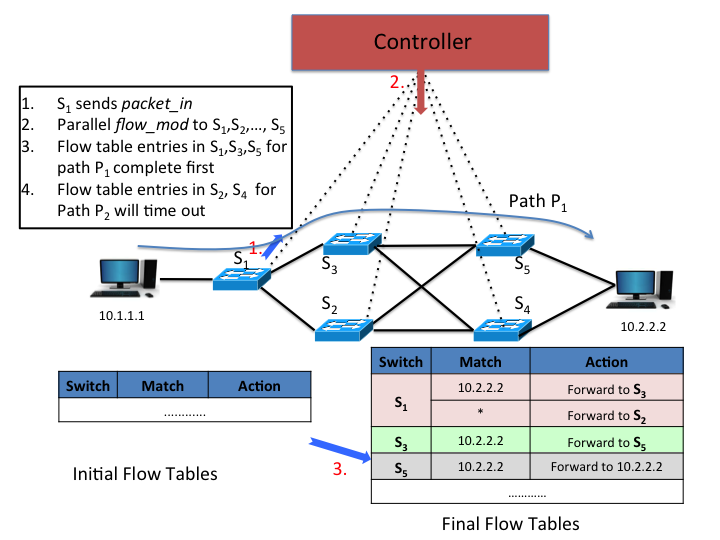
\includegraphics[width=3.5in]{figs/Mazu-mpath.png}
\caption{Exploiting parallel path setup}
\label{fig:mpath}
\end{figure}
%At the lowest level, Broadcom's SDK writes entries to specific addresses in the
%TCAM. If there are multiple entries, the one at the lower address always
%wins. But when you insert a single entry, the Broadcom SDK has no idea whether
%most of the entries you will insert later will be higher or lower
%priority. Nevertheless, it needs to pick an address. Whatever it picks it will
%be wrong for some input pattern. The update rates you see will depend on the
%specific heuristics used for picking addresses -- I do not know the
%specifics. The problem is that after inserting a small percentage of the
%entries, you will want to insert a new one between two existing entries, but
%they will be at adjacent addresses. So you have to make room by doing a
%"shuffle". It's no big deal if you only need to move one entry up or down by one
%address to make room, but as the device fills up you may need  to shuffle a
%large percentage of the entries to make room for the newcomer. Neither is it
%possible to game the system and make a lot of room for future entries because
%you don't know where they will need the room. Again, there are heuristics
%governing shuffles and how aggressively and proactively they are done -- I don't
%know the specifics of what they use. 

As we have seen in Figure x, \flowmod\ delay can be significantly affected by
other switch agent activities such as polling flow statistics.
%$flow\_mod$ time can be very preditable if all of
%them have the same priority. This is because no TCAM rule shuffles are needed.
%However, when rules have different priorities, different addresses are
%picked. Depending on the addresses picked, one may need to make room for new
%entries. Thus, shuffling may happen. \aditya{I don't think we want to use this
%  as a motivation because it contradicts what we are doing for flow engineering,
%  where we assume that the impact of priorities is predictable. why not use
%  pollstats and other uncontrolled activity as motivation??}  
%
To deal with unpredictible delay, we try to setup multiple paths. Data plane packets will
flow as soon as one path completes the setup. 
%\aditya{from here on out, the section was very hard to follow}
First, we illustrate our ideas using a simple example in
Figure~\ref{fig:mpath}. In this five-switch toplogy with switch
$S_1$,$S_2$,$\cdots$, $S_5$, host 10.1.1.1 originates a flow to host
10.2.2.2. Initially all flow tables are empty.
%entry that forward traffic to $S_2$. That is, $S_1$ delegates $packet\_in$
%processing to $S_2$. The reason for the delegation approach is to guard again the
%case that it takes sw1 a long time to install the rules. \emph{Essentially, we create
%two parallel paths even if a flow has a single ingress!} 
When sw1 receives the packet from 10.1.1.1, it will perform
the $packet\_in$ function (step 1). This can be done through our middlebox idea or
directly involve $S_1$'s CPU to generate a $packet\_in$ message and send to
controller. 
%The key point to note is that the $packet\_in$ message will have the
%incoming port information. For our middlebox idea, the incoming port ID can be
%stamped in the IPID field of the first packet before label switch it to the
%middlebox. 

%When the controller receives the $packet\_in$ message with the incoming port
%information, it knows that switch $S_2$ is acting as the delegate of switch
%$S_1$. 
In step 2 shown in the figure, the controller will set parallel
$flow\_mod$ messages to install rules for two paths: (1) path 1 is $S_1$,$S_3$,
$S_5$; (2) path 2 (except ingress) is $S_2$, $S_4$. In order for the controller to know
that $flow\_mod$ has appeared in a switch's hardware flow table, the controller
can send barrier messages to switches. Barrier messages request switch to notify
the controller when all rules before the barrier message is installed (not all
switch implement barrier message or implement it with a 
blocking semantics, i.e. barrier reply message is sent after the rule appears in
TCAM).  %\aditya{the sentence in paranthesis does not parse}

There are two cases. Case 1: suppose the controller
receives the barrier reply messages from all switches in path $P_1$ before path
2's $S_2$ and $S_4$. The controller will send a $packet\_out$ message to switch $S_1$. 
%The controller supplies the complete packet in the message. 
The first packet will be routed
through switch $S_3$ and $S_5$ to the destination. Our middlebox idea nicely
handles the case that multiple packets accumulate before the path setup
completes. Switch $S_2$ and $S_4$'s rule entries for path 2 will be timed out
since no traffic will follow. Case 2: path $P_2$'s $S_2$, $S_4$ comes back
first. Suppose $S_1$ also comes back. Then the controller will modify the rule
entry so that the action will direct traffic to path 2.   
% However, when the entry for 10.2.2.2 appears in $S_1$'s hardware flow
%table. Packets will match this high priority rule. So the flow from 10.1.1.1 to
%10.2.2.2 will experience a path switching. If we pick the two paths with similar
%latency, packet reordering should be easily handled at the destination. After
%the switching, rule entries at sw2 and sw4 will be timed out.

\program{prog:mflow-mpath}
    {Parallel Path Setup for Multiple Flows}
{
//$N$ flows, compute $K$ disjoint paths per flow \\
//$maxNEntries$: maximal additional entries we place in each switch \\
while ($i<K$) \{ \\
\> while ($j<N$) \{ \\
\>\>ComputeDisjointPath($flow_j$, $i$) //prune switches belong to more than \\
\>\>\> $maxNEntries$ paths \\
\>\>    $j = j+1$ \\
\> \} \\    
\> $i=i+1$ \\
}

Now we describe an algorithm that can work with concurrent setups of many
flows and each flow can have $K$ paths. For a target application such as
mobility, each UE demands a path with low data plane latency. Instead of
computing one shortest path (in terms of latency), we compute $K$ disjoint
shortest paths or $K$ paths such that each switch belongs to at most $L$ paths,
$L<K$. For simplicity, we consider the former. This problem is NP-hard. We can
take any known good approximation algorithm. We can concurrently setup these
$K$ paths in parallel as in our example. 

For joint solution of multiple flows, we will impose a constraint that no
switch should handle more than $MaxNEntries$ number of $flow\_mod$.  For
fairness, we compute one path for all flows before computing the second
joint path for all flow and so on.  The algorithm is shown in
Figure~\ref{prog:mflow-mpath}. 

%\li{add the algorithm pseudo code}

\iffalse
For mobility, we can compute K-paths per flow or jointly. (1) For per flow, lets
use K shortest paths (i.e. ECMP). These K paths should be disjoint or share
minimal number of switches. Lets use disjoint paths. (2) For joint solution of
multiple flows, we will have the same MaxNEntries constraint per switch. For
fairness, you can compute one path for all flows before computing the second
joint path for all flow, etc.  


Even while I was at Broadcom I had little visibility into how the switch guys'
software handled their TCAM. Now that I'm outside I have zero visibility (I work
on search, not on network infrastructure at Google). But I have a broad
explanation of what you see that I am pretty confident is correct. 
 
The API allows you to associate priorities with rules/entries. The API does not
let you tell the hardware how many lower priority or higher priority rules you
will insert in the future. Nor is this easy to figure out, so even if there were
such API, it would be hard to use. But this is exactly what the software would
need in order to ensure fast updates. A more realistic alternative API would be
to give all the entries at once - I don't know whether such a batch API is
available. 

At the lowest level, Broadcom's SDK writes entries to specific addresses in the
TCAM. If there are multiple entries, the one at the lower address always
wins. But when you insert a single entry, the Broadcom SDK has no idea whether
most of the entries you will insert later will be higher or lower
priority. Nevertheless, it needs to pick an address. Whatever it picks it will
be wrong for some input pattern. The update rates you see will depend on the
specific heuristics used for picking addresses -- I do not know the
specifics. The problem is that after inserting a small percentage of the
entries, you will want to insert a new one between two existing entries, but
they will be at adjacent addresses. So you have to make room by doing a
"shuffle". It's no big deal if you only need to move one entry up or down by one
address to make room, but as the device fills up you may need  to shuffle a
large percentage of the entries to make room for the newcomer. Neither is it
possible to game the system and make a lot of room for future entries because
you don't know where they will need the room. Again, there are heuristics
governing shuffles and how aggressively and proactively they are done -- I don't
know the specifics of what they use. 

One common property of all these TCAM shuffle algorithms is that they work
spectacularly well when entries have the same priority. Shuffles are not
needed. The Broadcom SDK is allowed to write the new entries to any available
TCAM address. 

Please let me know if anything you see contradicts this explanation - there may
be more going on, but usually the shuffles are the big update rate killer. 

Cheers,

Cristi



On Tue, Jan 21, 2014 at 12:59 PM, Aditya Akella <akella@cs.wisc.edu> wrote:
Hi Cristi,

One other question for you that has really been bugging us and we simple can't figure out what's going on. We did a bunch of experiments where we see bizarre and inconsistent results.

Expt 1: We conducted an experiment where we installed a burst of rules of size B of a certain priority pattern P. We measure total latency to install the rules:

1. B --> increasing priority: we see latencies really shoot up, with the burst taking almost 30s to install. This makes sense as perhaps each incoming higher priority rule is causing TCAM rearrangement (?)
2. B --> decreasing priority: we see high latencies too, over 20s to install. We did not expect this as we were hoping the latencies would be the same as B --> same priority.

Any thoughts on what may be going on? So we thought something weird is happening with low/high priorities, so we decided to run a bunch of experiments that played with the pattern of priorities. Here are a couple:

Expt 2: We installed ~700 each of alternating high and low priorities. We saw all rules with the higher priority were installed first (within ~1.5s in all) after which the low priority rules started to get inserted, which kind of makes sense except that the  low latency rule installation completed after 20s or more!

But:

Expt 3: If instead of sending the burst of about 700 above, we first sent 350 high priority rules, and then send a burst of 350 low priority rules after the first batch was installed, then the completion time of the latter is far far lower than what we see in Expt 2.

What on earth is going on? Can you shed some light in general on how Broadcom handles priorities? Is there some obvious issue we are missing out on?

\fi

\subsection{Rule Reordering}
\label{s:optimal}

Our measurements show that given rules of different priorities to be inserted at
a switch, the ``optimal'' order of rule insertion varies with switch platform
because of the difference in architecture and the workload the hardware is
optimized for. For Intel, the optimal order is to insert
rules in \emph{increasing} order of priority, whereas the \emph{opposite} is
true for Broadcom. Given this observation, Mazu controls the actual rule
insertion using the pattern that is optimal for the switch. 

We assume one-shot consistent updates~\cite{one-shot} are in use. In this case, new rules will not take effect unless all of them are installed. Therefore, Mazu can optimize the ordering without causing temporal policy violations. Mazu's techniques can also be adapted for other update schemes~\cite{mahajan13:hotnets}.

%\aditya{is there more to say here?} 

% \aditya{I'm not sure what our measurements show here. Is a particular insertion order better than another?}

% \aditya{Li and I were thinking that given a set of rules to insert into a switch, the idea would be to sort them in descending order of priority and insert. The intuition is that the higher priority rules inserted earlier will not be disturbed by later lower priority rules (in contrast if we change the order then a lower priority rule inserted earlier may have to be moved around to make room for a later higher priority rule).
% However, our experiments are inconclusive in this respect, correct? (we see that decreasing priority order has somewhat arbitrary performance, and shows abnormally high latency? Also when we interleave priorities we see all high priority inserted first.)
% So what is our story here?}

% LocalWords:  Broadcom Mazu


% LocalWords:  TCAMs OpenFlow SDK ACLs Mazu Broadcom
